% 原书 p.115–p.120（PDF p.123–p.128 上半）；本节为第 5 章 5.2 节（持续模）
% 说明：本文件延续 ch05a-s01.tex，不重复 \chapter；5.2 节开头位于 PDF p.123 中部。
\section{持续模（Persistence Module）}

% >>> p123
\begin{keytakeaways}
\begin{itemize}
  \item 几何图像：把一个 Morse 函数 $F$ 的临界值当作「过滤器」，只观察子水平集
        $\{F(x)<t\}$ 的同调，得到一族随 $t\in\R$ 变化的同调群。
  \item 数学工具：\textbf{持久 $\mathbf k$-模}由一族有限维 $\mathbf k$-模
        $\{V_t\}$ 与结构映射 $\{\iota_{s,t}:V_s\to V_t\}_{s\leqslant t}$ 组成，
        满足 $\iota_{t,t}=\mathbf 1$ 与 $\iota_{s,t}\circ\iota_{r,s}=\iota_{r,t}$；
        它等价于函子 $(\R,\leqslant)\to\mathrm{Vect}_{\mathbf k}$。
  \item 本节结论（正规形定理 5.2.1）：任意持久模分解为区间型模
        $\mathbf k_I$ 的直和 $\mathbb V\cong\bigoplus_{I\subset\R}\mathbf k_I$，
        且重数唯一；这就给出\textbf{条形码} $\mathbb B(\mathbb V)$。
  \item 定量含义：半无限条对应经典同调中「可见」的生成元，有限条对应经典同调中
        「不可见」的生成元——后者正是 Morse 同调所丢失、而持续模所保留的信息。
\end{itemize}
\end{keytakeaways}

持续模是一种代数结构，其发明部分是为了解决上一节末尾第 (iii) 点所提到的问题——在
Morse 理论中，如何系统地使用临界值？关键想法是用临界值来细化我们的计算对象：不去
计算整个流形的 Morse 同调群，而只计算临界值之下的「子水平集」。

一般而言，持续模由 G. Carlsson 与 A. Zamorodian [248] 引入，亦称持续同调理论。
另可参看 H. Edelsbrunner、D. Letscher 与 A. Zomorodian 的文献 [70]。更新的进展见
[241, 174, 45, 182]。他们的动机往往来自拓扑学的进路，用以处理数据云（由数据云过渡
到标准的拓扑框架——一族参数化的单形）。下面我们将从 Morse 理论的角度来展示这一点。

% [Tutor Note: 术语/记号依据——原文两处把 Zomorodian 拼作 Zamorodian / Zomorodian
% （同一作者的不同拼写），译文照原文保留。持久同调（persistent homology）与持续模
% （persistence module）是同一理论的不同表述：前者着眼于同调群随参数变化的「条」，
% 后者着眼于代数结构本身。本书偏好后者，因为它便于做代数运算。]

严格地说，考虑「过滤的」Morse 同调，即对任意 $t\in\R$，计算
\begin{equation}\tag{5.11}
\mathrm{HM}_*\left(\{F(x)<t\};\mathbf k\right).
\end{equation}
注意定理 5.1.2 仍然适用，因此
$\mathrm{HM}_*(\{F(x)<t\};\mathbf k)$ 计算子水平集
$\{F(x)<t\}\subset X$ 的经典同调群，即
$H_*(\{F(x)<t\};\mathbf k)$。此外，若 $s\leqslant t$（$s,t\in\R$），则包含映射
$\{F(x)<s\}\subset\{F(x)<t\}$ 诱导过滤 Morse 同调上的 $\mathbf k$-线性映射
\begin{equation}\tag{5.12}
\iota_{s,t}:\mathrm{HM}_*(\{F(x)<s\};\mathbf k)
\to\mathrm{HM}_*(\{F(x)<t\};\mathbf k).
\end{equation}
注意此映射可以既不是单射也不是满射（见例 5.2.1）。然而 $\iota_{s,t}$ 满足如下
「函子性质」：对任意 $t\in\R$，映射 $\iota_{t,t}=\mathbf 1$；对任意
$r\leqslant s\leqslant t\in\R$，有 $\iota_{s,t}\circ\iota_{r,s}=\iota_{r,t}$。

% [Tutor Note: 易错预警——(5.11) 用的是严格不等式 $\{F(x)<t\}$，因此当 $t$ 恰为
% 临界值时子水平集不发生变化：关键的跳跃发生在「$t$ 越过临界值」的瞬间。这也解释了
% 例 5.2.1 中为何按 $t\leqslant t_1$、$t_1<t\leqslant t_2$ 分段。若改用
% $\{F(x)\leqslant t\}$，所有区间的端点开闭性会整体改变，但条形码作为多重集不变。]

与上一节的 Morse 同调群类似，过滤 Morse 同调也是可计算的。让我们从这一新视角重新
审视例 5.1.10 中的心形圆周。

\begin{wexam}{5.2.1}
考虑图 5.11 中的心形圆周 $X$。设 $F:X\to\R$ 为高度函数，其中临界值
$F(p_0)=t_1$、$F(q_0)=t_2$、$F(p_1)=t_3$、$F(q_1)=t_4$ 满足
$t_1<t_2<t_3<t_4$。

% >>> p124
\begin{figure}[htbp]
  \centering
  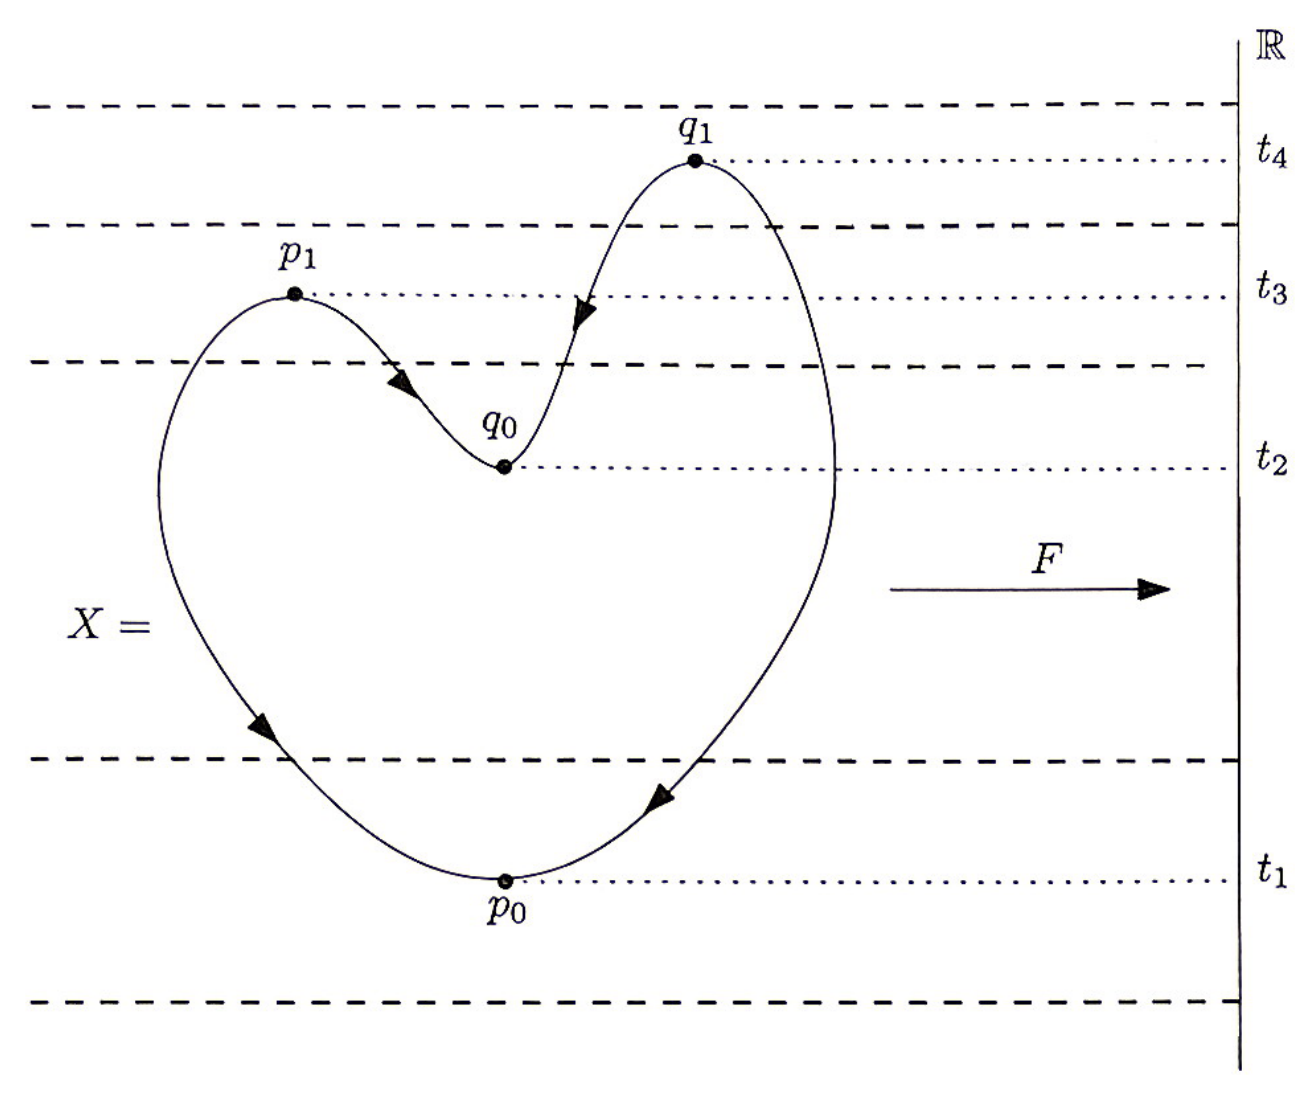
\includegraphics[width=0.70\linewidth]{figures/fig_p124_1.png}
  \caption*{图 5.11\quad 心形圆周的不同子水平集（原书 p.116, Figure 5.11；
  PDF p.124）}
\end{figure}

\begin{enumerate}[label=(\roman*)]
  \item 当 $t\leqslant t_1$ 时，$\{F(x)<t\}=\varnothing$，故
        $\mathrm{HM}(\{F(x)<t\};\mathbf k)=0$。
  \item 当 $t_1<t\leqslant t_2$ 时，子水平集 $\{F(x)<t\}$ 形变收缩到点 $p_0$，故
        $\mathrm{HM}_0(\{F(x)<t\};\mathbf k)=\mathbf k\langle p_0\rangle$，而其他
        次数 $\mathrm{HM}_{*\ne0}(\{F(x)<t\};\mathbf k)=0$。
  \item 当 $t_2<t\leqslant t_3$ 时，子水平集 $\{F(x)<t\}$ 含两个连通分支，其中每个
        在拓扑上平凡，故
        \begin{equation}\tag{5.13}
        \mathrm{HM}_0(\{F(x)<t\};\mathbf k)
        =\mathbf k\langle p_0,q_0\rangle
        =\mathbf k\langle p_0,p_0+q_0\rangle,
        \end{equation}
        而其他次数仍为 $\mathrm{HM}_{*\ne0}(\{F(x)<t\};\mathbf k)=0$。
  \item 当 $t_3<t\leqslant t_4$ 时，前一情形的两个分支合并，故
        $\mathrm{HM}_0(\{F(x)<t\};\mathbf k)=\mathbf k\langle p_0\rangle$
        （因为生成元 $p_0+q_0$ 被一个新生的生成元 $p_1$ 在 Morse 边界算子下杀死），
        其他次数仍为 $0$。
  \item 当 $t>t_4$ 时，子水平集是整个流形 $X$，故由 (5.10) 有
        $\mathrm{HM}_0(\{F(x)<t\};\mathbf k)=\mathbf k\langle p_0\rangle$ 与
        $\mathrm{HM}_1(\{F(x)<t\};\mathbf k)=\mathbf k\langle p_1-q_1\rangle$。
\end{enumerate}

作为对比，定义在 (5.9) 中的标准 Morse 同调 $\mathrm{HM}_*(F;\mathbf k)$ 只看到
$t>t_4$ 的情形。此外，对 $s\in(t_1,t_2)$ 与 $t\in(t_2,t_3)$（从而 $s<t$），
(5.12) 中定义的映射是从 $\mathbf k\to\mathbf k^2$，不是满射；而
% >>> p125
对 $s\in(t_2,t_3)$ 与 $t\in(t_3,t_4)$（从而 $s<t$），(5.12) 中定义的映射是从
$\mathbf k^2\to\mathbf k$，不是单射（其核由 $\mathbf k\langle p_0+q_0\rangle$
给出）。\hfill$//$
\end{wexam}

% [Tutor Note: 易错预警——注意例 5.2.1 (iii) 中的等式
% $\mathbf k\langle p_0,q_0\rangle=\mathbf k\langle p_0,p_0+q_0\rangle$：
% 这只是「同一子空间的两组基」，不是同调类的等同。选基 $\{p_0,p_0+q_0\}$ 是为
% 了让 (iv) 中的边界算子作用「上三角化」，从而条形码的端点可以直接读出（见注 5.2.3）。
% 若坚持用 $\{p_0,q_0\}$，则 $\partial_1$ 的矩阵不是上三角形，条形码的「出生/死亡」
% 会被基变换搅乱。]

下面的定义是过滤 Morse 同调群 (5.11) 的抽象代数表述。

\begin{wdefn}{5.2.1}
一个\textbf{持久 $\mathbf k$-模}是一个由如下数据组成的包裹
\[
\mathbb V=\left(\{V_t\}_{t\in\R},\ 
\{\iota_{s,t}:V_s\to V_t\}_{s\leqslant t\in\R}\right),
\]
其中 $V_t$ 对任意 $t\in\R$ 是有限维 $\mathbf k$-模，而 $\iota_{s,t}$ 是
$\mathbf k$-线性映射，满足 $\iota_{t,t}=\mathbf 1_{V_t}$，且对任意
$r\leqslant s\leqslant t\in\R$ 有 $\iota_{s,t}\circ\iota_{r,s}=\iota_{r,t}$。
这些映射 $\{\iota_{s,t}\}_{s\leqslant t\in\R}$ 称为 $\mathbb V$ 的
\textbf{结构映射}（structure maps）。
\end{wdefn}

\begin{wrem}{5.2.1}
也可以把持久 $\mathbf k$-模重新表述为从 $(\R,\leqslant)$ 到
$\mathrm{Vect}_{\mathbf k}$ 的函子，其中 $(\R,\leqslant)$ 表示如下范畴：对象是
元素 $r\in\R$，而 hom-集定义为
\[
\hom_{\R}(r,s)=
\begin{cases}
\varnothing, & \text{若}\ r>s,\\
\{*\}, & \text{若}\ r\leqslant s.
\end{cases}
\]
这里，$\mathrm{Vect}_{\mathbf k}$ 表示有限维 $\mathbf k$-模的范畴。
\end{wrem}

\begin{wexam}{5.2.2}
对 Morse 函数 $F:(X,g)\to\R$（其中 $g$ 是 $X$ 上的通有度量），过滤 Morse 同调群
构成一个持久 $\mathbf k$-模：
\[
\mathbb V_F:=\left(\left\{V_t:=\mathrm{HM}_*\left(\{F(x)<t\};\mathbf k\right)
\right\}_{t\in\R},\ 
\left\{\iota_{s,t}:V_s\to V_t\right\}_{s\leqslant t\in\R}\right).
\]
这里要强调，上面的持久 $\mathbf k$-模 $\mathbb V_F$ 依赖于 Morse 函数 $F$ 的选取。
当 $F$ 变化时 $\mathbb V_F$ 如何变化，是一个非常有意义的问题。我们留给有兴趣的读者
自行探索，然后查阅文献 [45]（关键词——\emph{交错距离}（interleaving distance））。
\hfill$//$
\end{wexam}

% [Tutor Note: 含糊点拨——$\mathbb V_F$ 的「函子性」来自 (5.12) 的合成性质；而
% 「当 $F$ 变化时 $\mathbb V_F$ 如何变化」的完整答案是稳定性定理：两个 Morse 函数
% 之间的 $C^0$-距离控制其条形码之间的瓶颈距离（bottleneck distance）。本书不展开，
% 但 6.2 节会用到其推论（定理 6.2.1）。]

下面的例子说明持久 $\mathbf k$-模（在代数意义上）最基本的情形。

\begin{wexam}{5.2.3}
固定一个区间 $I\subset\R$，其中 $I$ 可以是有限区间或半无限区间，考虑如下以
$\mathbf k_I$ 记之的持久 $\mathbf k$-模
\[
(\mathbf k_I)_t:=
\begin{cases}
\mathbf k, & \text{若}\ t\in I,\\
0, & \text{其他情形}.
\end{cases}
\]
对 $\R$ 中的 $s\leqslant t$，仅当 $s,t\in I$ 时置
$\iota_{s,t}=\mathbf 1_{\mathbf k}$，否则置 $\iota_{s,t}=0$。所得的持久
$\mathbf k$-模称为（区间 $I\subset\R$ 上的）\textbf{区间型}持久 $\mathbf k$-模。
\hfill$//$
\end{wexam}

与任何代数对象一样，持久 $\mathbf k$-模容许分解（分解为不可分解块的直和）。下面的
结果是精确的陈述，它
% >>> p126
是持久 $\mathbf k$-模理论的两个主要结果之一。另一个结果称为\emph{稳定性定理}或
\emph{等距定理}，本书不会显式涉及，但它有助于导出 6.2 节中的定理 6.2.1。关于第二个
定理的更多细节，见 [182] 的 2.2 节与 2.3 节。

\begin{wthm}{5.2.1}（正规形；[182] 中的定理 2.1.2）
由定义 5.2.1 给出的任意持久 $\mathbf k$-模 $\mathbb V$ 都可以分解为例 5.2.3 中
区间型持久 $\mathbf k$-模的直和
\begin{equation}\tag{5.14}
\mathbb V\cong\bigoplus_{I\subset\R}\mathbf k_I.
\end{equation}
此外，在重排意义下，(5.14) 中的区间 $I$（连同其重数）是唯一的。
\end{wthm}

% [Tutor Note: 含糊点拨——定理 5.2.1 通常称为「持续模的结构定理」或「正规形定理」。
% 证明思路是对 $\mathbb V$ 的分次块作 Gauss 消去式的基变换（即把结构映射矩阵化为
% 阶梯形），这也解释了为何要求每个 $V_t$ 有限维。该定理对「逐点有限维」的持久模成立；
% 若 $V_t$ 是无限维 Banach 空间，则区间分解一般失效，需要额外假设。]

由于定理 5.2.1 的第二个结论，对定理 5.2.1 中的每个持久 $\mathbf k$-模
$\mathbb V$，由 (5.14) 分解中出现的所有区间 $I$ 构成的多重集（即允许元素重复出现的
集合）是良定义的，记作 $\mathbb B(\mathbb V)$，并称为 $\mathbb V$ 的
\textbf{条形码}（barcode）。

\begin{wrem}{5.2.2}
定理 5.2.1 蕴含 $\mathbf k_{(0,2]}$ 与
$\mathbf k_{(0,1]}\oplus\mathbf k_{(1,2]}$ 作为两个持久 $\mathbf k$-模是不同的
（因为它们的条形码不同），尽管对任意 $t\in\R$，它们的纤维相同。这说明持久
$\mathbf k$-模的数据包裹中，结构映射 $\{\iota_{s,t}\}_{s\leqslant t\in\R}$ 也是
本质的。
\end{wrem}

% [Tutor Note: 易错预警——注 5.2.2 是「持久模比一族同调群更强」的核心例证：两族的
% 逐点纤维 $\{V_t\}$ 完全相同，但结构映射不同，故条形码不同。这也是为什么持续同调
% 能区分「同调不可见」的生成元，而经典同调不能。]

\begin{wexam}{5.2.4}
对例 5.1.10 中的持久 $\mathbf k$-模 $\mathbb V_F$（它来自例 5.2.1 的详细计算），
其条形码为
\[
\mathbb B(\mathbb V_F)=\left\{(t_1,+\infty),\ (t_2,t_3),\ (t_4,+\infty)\right\}.
\]

% [Tutor Note: 原文疑误——原文说「例 5.1.10 中的持久 $\mathbf k$-模 $\mathbb V_F$」，
% 但 $\mathbb V_F$ 是在例 5.2.2 中定义的（例 5.1.10 只定义了 Morse 同调群）。
% 译文照原文保留，已在 review_ch05a.md 记录。另注意条形码 (5.14) 中的区间是
% 半开区间 $I=(a,b]$ 或 $(a,+\infty)$，其开闭端点由 (5.11) 中严格不等号的选择决定；
% 不同文献的约定可能相差一个端点，但条形码的多重集整体不变。]

找出这个条形码的一个办法，是跟踪例 5.2.1 中各生成元的「生」与「死」。例如
(5.13) 中的生成元 $p_0+q_0$ 在 $t$ 越过 $t_2$ 时出生，并在 $t$ 越过 $t_3$ 时在
同调中死亡（此时 $p_1$ 出现并杀死 $p_0+q_0$）。再如，生成元 $p_0$ 在 $t$ 越过
$t_1$ 时出生，且永不死亡。

重要的是，$\mathbb B(\mathbb V_F)$ 中的半无限区间对应于经典同调群中
\emph{同调可见的}生成元；$\mathbb B(\mathbb V_F)$ 中的有限区间对应于经典同调群中
\emph{同调不可见的}生成元，即在经典同调群 $\mathrm{HM}_*(F;\mathbf k)$ 中看不到的
那些生成元。\hfill$//$
\end{wexam}

\begin{wrem}{5.2.3}
我们在例 5.2.4 中求出条形码的方式，对过滤 Morse 同调群基的选取相当敏感（见 (5.13)）。
一个「容许的」基由这样的元素组成：它们能帮助我们把子空间 $\ker(\partial_*)$ 直接
分裂为 $\operatorname{im}(\partial_{*+1})$ 及其补空间。构造容许基只遵循一条规则：
基元素的任何线性组合都不能严格降低它们在 Morse 函数 $F$ 下的赋值。例如，如 (5.13)
所示，我们偏好基元素 $\{p_0,p_0+q_0\}$ 而不是 $\{q_0,p_0+
% >>> p127
q_0\}$，因为
\[
F\left((-1)\cdot q_0+1\cdot(p_0+q_0)\right)
=F(p_0)=t_1<t_2=F(q_0)\ \text{或}\ F(p_0+q_0).
\]
换言之，$\{q_0,p_0+q_0\}$ \emph{不是}容许基。这里，$p_0+q_0$ 在 $F$ 下的赋值定义为
$\max\{F(p_0),F(q_0)\}(=t_2)$（总是取「最大」）。关于基选取的更自然的解释，
特别是在链复形层面，见 8.2 节。
\end{wrem}

% [Tutor Note: 术语/记号依据——注 5.2.3 中的「赋值」（valuation）指
% $\operatorname{val}(x):=\max\{F(p)\mid p\ \text{出现在}\ x\ \text{的展开中}\}$；
% 容许基的要求是：对任意基元素 $x,y$ 与系数 $c$，有
% $\operatorname{val}(x+cy)\leqslant\max\{\operatorname{val}(x),
% \operatorname{val}(y)\}$，即「不能靠线性组合降低赋值」。这与持久模的矩阵约化
% 算法（Gauss 消去）中「按赋值从小到大消元」的做法是同一回事。]

下面是一个练习，用来练习如何从过滤 Morse 同调群中提取条形码。

\begin{wexer}{5.2.1}（[183] 中的 2.4 节）
对下图 5.12 中的曲面 $\Sigma_2=\T^2\#\T^2$（二维的！），它被视为两个环面的连通和。
取高度函数 $f:\Sigma_2\to\R$ 作为其上的 Morse 函数。计算/画出由过滤 Morse 同调群
给出的持久模 $\mathbb V_f$ 的条形码。请仔细标注条形码中各条的端点。
\end{wexer}

\begin{figure}[htbp]
  \centering
  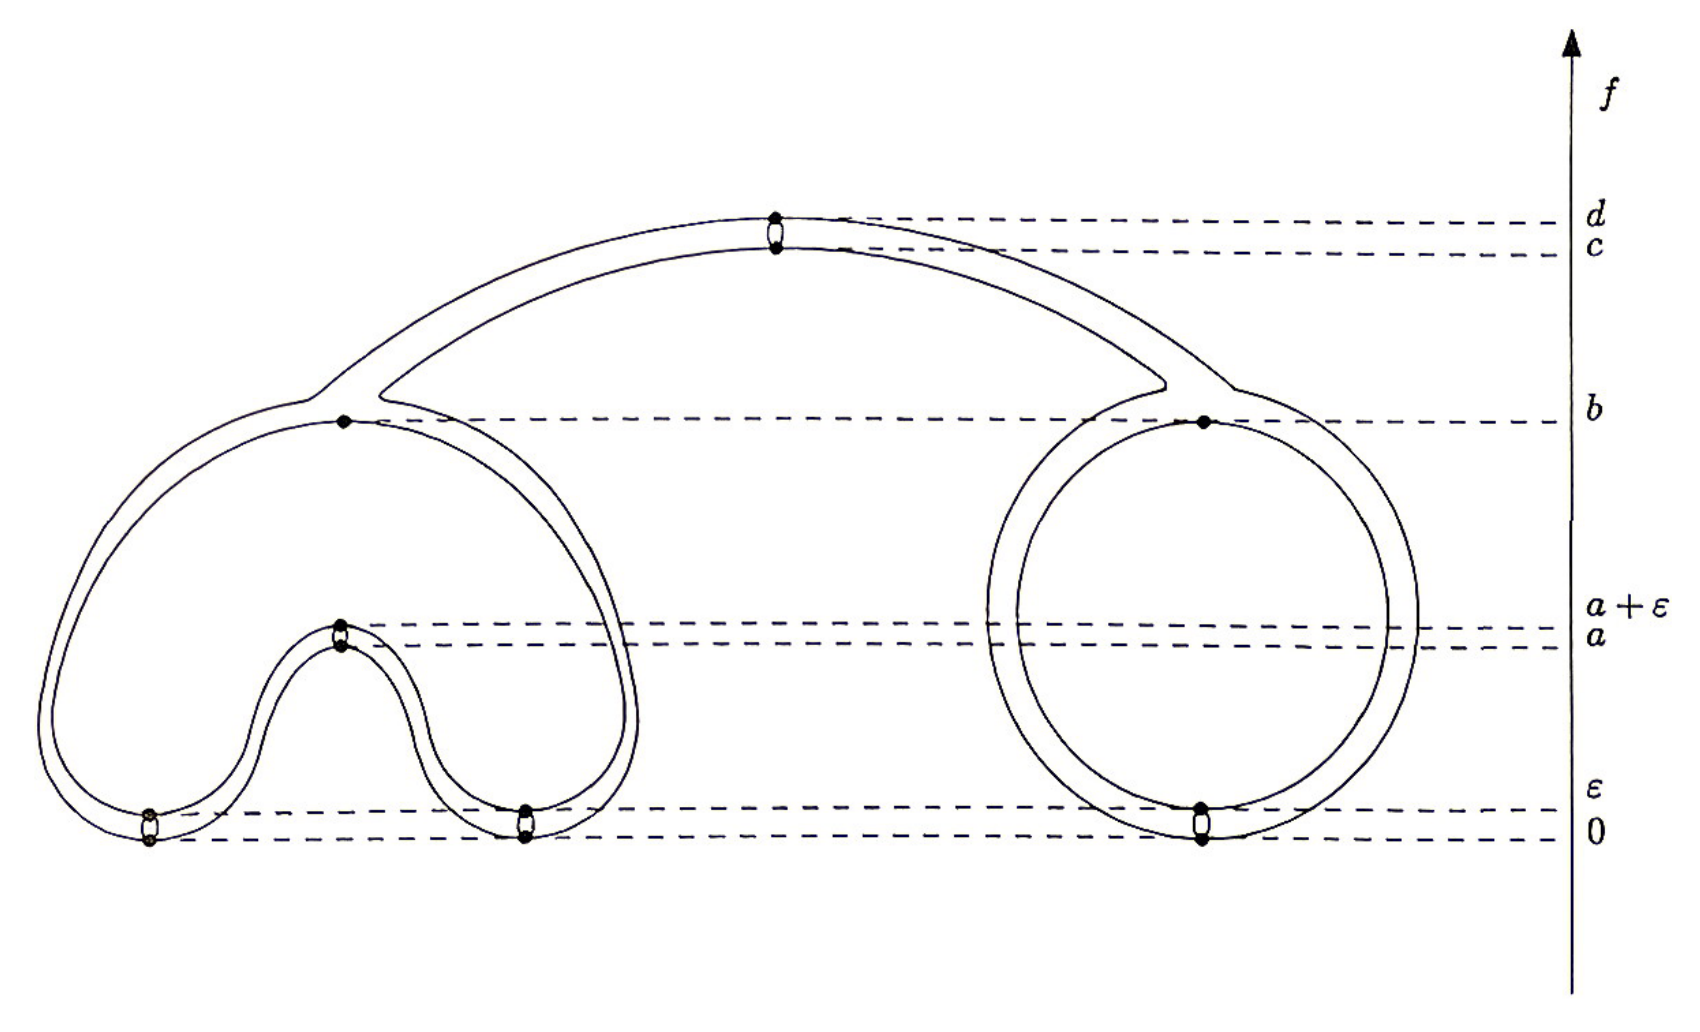
\includegraphics[width=0.9\linewidth]{figures/fig_p127_1.png}
  \caption*{图 5.12\quad 曲面 $\Sigma_2=\T^2\#\T^2$ 与高度函数
  $f:\Sigma_2\to\R$（原书 p.119, Figure 5.12；PDF p.127）}
\end{figure}

下面的练习引入另一个重要概念，它帮助持久模之间彼此「交流」。

\begin{wexer}{5.2.2}
对两个持久模
$\mathbb V=(\{V_t\}_{t\in\R},\{\iota^{\mathbb V}_{s,t}:V_s\to V_t\}_{s\leqslant t\in\R})$
与
$\mathbb W=(\{W_t\}_{t\in\R},\{\iota^{\mathbb W}_{s,t}:W_s\to W_t\}_{s\leqslant t\in\R})$，
持久模之间的\textbf{态射} $f:\mathbb V\to\mathbb W$ 是一族 $\R$-线性的线性映射
$f=\{f_t:V_t\to W_t\}_{t\in\R}$，使得对任意 $s\leqslant t$ 有
$f_t\circ\iota^{\mathbb V}_{s,t}=\iota^{\mathbb W}_{s,t}\circ f_s$。证明：对区间型
持久 $\mathbf k$-模 $\mathbf k_{(a,b)}$ 与 $\mathbf k_{(c,d)}$，
% >>> p128
存在非零持久态射从 $\mathbf k_{(a,b)}$ 到 $\mathbf k_{(c,d)}$，当且仅当
$c\leqslant a$ 且 $a<d\leqslant b$。
\end{wexer}

% [Tutor Note: 易错预警——练习 5.2.2 的条件 $c\leqslant a<d\leqslant b$ 正是
% 区间 $(a,b)$ 与 $(c,d)$ 之间「有重叠且后者的左端点不晚于前者」的刻划，它保证
% 结构映射在两端能接上。该练习是「交错距离」定义的代数基础：两个持久模的条形码
% 若在 Hausdorff 意义下接近，就存在一对方向相反、满足平移关系的态射。]

% [Tutor Note: 原文疑误（轻微）——末段原文作 "homological invisible generators"，
% 从上下文看应为 "homologically invisible generators"（同调不可见的生成元）。
% 译文按语义译出，不影响数学内容。]

为结束本节，我们（再次）强调：由过滤同调群得到的持久模丰富了经典同调理论，因为它使
同调不可见的生成元得以被考察。
